

We  now discuss   syntax and semantics of  our specifications, and illustrate through examples.

\subsection{Specifications syntax }

Our specifications language % \SpecLang,  
 supports scoped invariants,  and  method specifications, and sequences.
 
\begin{definition} [Specifications]  { } %  We define the \emph{syntax} of \SpecLang and well-frmedness:
\noindent

\begin{itemize}
\item
The syntax of specifications, $S$, is given below
\label{f:holistic-syntax}
\[
\begin{syntax}
\syntaxElement{S}{ }
		  {\syntaxline
                               %   {  \OneStateQ {\overline {x:C}} {A} }	
				{ \TwoStatesN {\overline {x:C}} {A}  }
				%  {\mprepost{A}{C}{m}{x}{C}{A} }
%		 \endsyntaxline
% 		}
%  		{
% 		\syntaxline
 				{\mprepostN{A}{p\ C}{m}{x}{C}{A} {A}}%{A[\!\![ \,C\!::\!m(\overline{x:C})\,]\!\!] A }}
				{S\, \wedge \, S}
		 \endsyntaxline
 		}
\endSyntaxElement\\
\syntaxElement{p}{ } 
 	 {\syntaxline
                                  {\  \ \ \  \prg{private} \ } 	
				 {\   \prg{public} \ } 	
		 \endsyntaxline
 		}
\endSyntaxElement 
\end{syntax}
\]

\item
{\emph{Well-formedness},  $\vdash S$,  is   defined by cases on $S$:\\
  $\strut \ \  \vdash {\TwoStatesN {\overline {x:C}} {A}}$\ \  if  \ \ $\fv(A)\subseteq\{  \overline x \}$;\\
  % \ \ \ \ \ \ \ \ \ \ \ 
% $\vdash {\TwoStatesQ {\overline {x:C}} {A} {A'}}$  if    $\fv(A), \fv(A')\subseteq \{ \overline x \}$; \\
% $\strut \ \  \vdash {\mprepost{A}{C}{m}{x}{C}{A'} }$   if      $\fv(A')\subseteq  \fv(A)\cup \{\prg{res}, \prg{this}, \overline x\}$; \\
 $\strut \ \  \vdash {\mprepostN{A}{p\ C}{m}{x}{C}{A'} {A''}}$ \ \   if  \ \    $\fv(A')$, $\fv(A'')\subseteq  \fv(A)\cup \{\prg{res}, \prg{this}, \overline x\}$; \\
 $\strut \ \  \vdash S\, \wedge \, S'$\ \  if \ \  $\vdash S$   and   $\vdash S'$.  
}
\end{itemize} 
\end{definition}

We now consider some examples.

% DO NOT ERASE - we may resurrect --  currently not  requiring these 
% {\begin{example}[One-state Invariants]
% \label{example:oneState}
%  $S_{10}$  guarantees   that  the balance is never negative:
%  \\
%   \begin{tabular}{lcll}
%$\strut \ \ \ \ \ \ \ \ S_{10}$ & $\triangleq$   & ${\OneStateQ {\prg{a}:\prg{Account}} {\prg{a.\balance} \geq 0}}$
% \end{tabular}
%  
% \end{example}
%}

{
 \begin{example}[Scoped Invariants]
 \label{example:twostate}
  % 
 $S_5$  guarantees   that   non-null passwords do not change:
 \\
 \begin{tabular}{lcll}
$\strut \ \ \ \ \ \ \ \ S_5$ & $\triangleq$   & ${\TwoStatesN {\prg{a}:\prg{Account}.\prg{p}:\prg{Password}}  {\prg{null}\neq \prg{p}=\prg{a.\password}}} $  \end{tabular}
 \end{example} 
 }
 
{ \begin{example}[Method Specifications]
 \label{example:mprepostl}
$S_6$ below  guarantees that
\prg{transfer} does not affect the balance of accounts different  from the receiver or argument, and  if the password supplied is not that of the receiver, then no account's balance is affected.  \
$S_7$ guarantees that if the password supplied is that of the receiver, the correct amount is transferred from the receiver to the destination.
\ 
 $S_8$ guarantees that \prg{set} preserves the protectedness of a password.
\ 
 $S_9$ guarantees that  \prg{buy} does not decrease  the balance of the shop's account provided that its  password  is protected from the buyer.
% The specifications from below describe properties ot the methods \prg{set}  and \prg{transfer}:
\\
\small{
{\sprepost
		{\strut \ \ \ \ \ \ \ \ \ S_6} 
		{ a:\prg{Account}\wedge  a.\prg{\balance}=b \wedge
		(\prg{dst}\neq a\neq\prg{this} \vee \prg{pwd'}\neq a.\prg{\password})}
	               {\prg{public Account}} {\prg{transfer}} {\prg{dst}:\prg{Account},\prg{pwd'}:\prg{Password},\prg{amt}:\prg{int}}
		{ a.\prg{\balance}=b}
}
\\
{\sprepost
		{\strut \ \ \ \ \ \ \ \ \ S_7} 
		{ % b,b':\prg{int} \wedge  
		\prg{this}\neq \prg{dst}\wedge \prg{this}.\prg{\balance}=b \wedge  \prg{dst}.\prg{\balance}=b' }
		  {\prg{public Account}} {\prg{transfer}} {\prg{dst}:\prg{Account},\prg{pwd'}:\prg{Password},\prg{amt}:\prg{int}}
		{\prg{this}.\prg{\balance}=b-\prg{amt} \wedge \prg{dst}.\prg{\balance}=b'+\prg{amt}}
}
\\
{\sprepost
		{\strut \ \ \ \ \ \ \ \ \ S_8} 
		{  a:\prg{Account}\wedge
		 \inside{a.\prg{\password}}}
		{\prg{public Account}} {\prg{set}} {\prg{pwd'}:\prg{Password}}
		{ \inside{a.\prg{\password}}}
}
\\
{\sprepost
		{\strut \ \ \ \ \ \ \ \ \ S_9} 
		{ %a:\prg{Account}\wedge
		 \protectedFrom{\prg{this}.\prg{\myAccount}.\prg{pwd}} {\prg{buyer}} \wedge \prg{this}.\prg{\myAccount}.\prg{\balance}=b
		 }
		{\prg{public Shop}} {\prg{buy}} {\prg{buyer}:\prg{external}, \prg{anItem}:\prg{Item} }
		{ 
		  \protectedFrom{\prg{this}.\prg{\myAccount}.\prg{pwd}} {\prg{buyer}} \wedge \prg{this}.\prg{\myAccount}.\prg{\balance}\geq b
		 }
}
}
%\\
%{\sprepost
%		{\strut \ \ \ \ \ \ \ \ \ S_{9}}
%		 {% a:\prg{Account}\wedge 
%		 a.\prg{password}\neq \prg{pwd'} \wedge a.\prg{\balance}=b}
%				       {\prg{Account}} {\prg{transfer}} {\prg{dst}:\prg{Account},\prg{pwd'}:\prg{Password},\prg{amt}:\prg{int}}
%		{ a.\prg{\balance}\geq b}
%}
%resp that the \balance of any account ...TODO ... explain ...
\end{example}
}

\subsection{Semantics of our specifications}

\red{ NOTE I deleted  Arising. Also deleted  GloballyReachable -- kept it for $\forall$ in assertions -- but perhaps not needed either.}
 
\footnoteSD{TODO motivate;
Here what we had: As discussed in \S \ref{s:approach}, 
{open world specifications need to be able to provide}
guarantees which hold
during execution of an internal, 
known, trusted module $M$ when linked together with any
unknown, untrusted, module $M_{ext}$. These guarantees need only hold 
when the external module is executing; we are not concerned if they are
temporarily broken by the internal module. Therefore, we are only interested in states where the
executing object (\prg{this}) is an external object. 
To express our focus on external states, we define the  \emph{external states semantics}, of the form 
$\reduction{M_{ext}}{M}{\sigma}{\sigma'}$, where $M_{ext}$ is the external
module, and $M$ is the internal module, and where we
collapse all internal steps into one single step.
}
% Temporarily hide
% we no longer require arising 
%{{Our specifications  describe  properties of states which \emph{arise} from the execution of our module combined with other, external modules, and
%starting at an \emph{intitial} state. %A state $\sigma$ is \emph{arising},}  written $\arising{\sigma}{M}$, {if it  may arise}  % by observable states} 
%%by execution
%% starting at some initial configuration:
%
%
%\begin{definition}[Arising  States]
%\label{def:arising}
%For modules $\overline M$ we define arising  states as follows:
%
%\begin{itemize}
%\itemWe  now define   syntax and semantics of  our specifications, and illustrate through examples.
%
Our specification language % \SpecLang,  
 supports scoped invariants,   method specifications, and {conjunctions}. 
\begin{definition} [Specifications Syntax]     We define the syntax  of  specifications, $S$:
\label{f:holistic-syntax}
\[
\begin{syntax}
\syntaxElement{S}{ }
		  {\syntaxline
                               %   {  \OneStateQ {\overline {x:C}} {A} }	
				{ \TwoStatesN {\overline {x:C}} {A}  }
				%  {\mprepost{A}{C}{m}{x}{C}{A} }
%		 \endsyntaxline
% 		}
%  		{
% 		\syntaxline
 				{\mprepostN{A}{p\ C}{m}{y}{C}{A} {A}}%{A[\!\![ \,C\!::\!m(\overline{x:C})\,]\!\!] A }}
				{S\, \wedge \, S}
		 \endsyntaxline
 		}
\endSyntaxElement\ 
\syntaxElement{p}{ } 
 	 {\syntaxline
                                  {\  \ \ \  \prg{private} \ } 	
				 {\   \prg{public} \ } 	
		 \endsyntaxline
 		}
\endSyntaxElement 
\end{syntax}
\]



% \end{itemize} 
\end{definition}

Def. \ref{f:holistic-wff}  describes well-formedness of specifications, $\vdash S$.
 We require for  scoped invariants, that the assertion is encapsulated, and that  its free variables  are bound by the quantifier. For method specifications, that the three assertions are $Stbl^+$, that the invariant part is encapsulated, that \prg{res} and \prg{this} are not in the formal parameters, that the free variables in the postcondition are either formal parameters or free  in the precondition, and similar for the invariant part.
%precondition's free variables all appear in the formal parameters or 
%{\emph{Well-formedness}},  $\vdash S$,  is   defined by cases on $S$:\\
%  $\strut \ \  \vdash {\TwoStatesN {\overline {x:C}} {A}} \ \ \ \triangleq\  \ \ \fv(A)\subseteq\{  \overline x \}\,\wedge\, {M \vdash \encaps {\sdN{\overline {x: C}} \wedge A}} $;\\
% $\strut \ \  \vdash {\mprepostN{A}{p\ C}{m}{y}{C}{A'} {A''}}\ \ \ \triangleq\  \ \  \exists \overline x, \overline {C'}.[ $\\
%  $\strut \hspace{1cm}  \sdN{\prg{res}\notin \overline{x}, \overline{y}}\,  \wedge\,  \ \sdN{\fv(A_0)\subseteq \overline{x},\overline y, \prg{this}}\   \wedge \fv(A')\subseteq  \fv(A),\prg{res}\   \wedge\  \fv(A'')\subseteq  \sdN{\overline{x}} $\\
%  $\strut \hspace{1cm}\wedge\  \Pos A\, \wedge\, \Pos {A'}\, \wedge \,\Pos {A''}\, \wedge  \,  M \vdash \encaps  {\overline {x: C'} \wedge A''}\ \ \  ]$ \\
%  $\strut \ \   \vdash S\, \wedge \, S' \ \ \triangleq \ \  \vdash S\, \wedge\, \vdash S'  $.  

 



\label{ssect:sem}
% \subsection{Specifications Semantics}

  
To give the semantics of specification we first \sdred{define quadruples involving states rather than statements}:
${\satAssertQuadruple  \Mtwo  M     {A} \sigma {A'} {A''} }$ 
  says that   if $\sigma$ satisfies $A$, then any terminating execution of its continuation (${\leadstoBoundedStarFin { \Mtwo\madd M}{\sigma}  {\sigma'} }$) will satisfy $A'$, and
 any intermediate reachable external state (here $\sigma''$) will satisfy $A''$. 
In  $A'$, we replace $A$'s free variables by their denotation in $\sigma$.

 
\begin{definition} \label{def:hoare:sem}
For modules $\Mtwo$, $M$, state $\sigma$, and assertions $A$, $A'$ and  $A''$, we define:
\begin{itemize}
\item
$ {\satAssertQuadruple  \Mtwo  M     {A} \sigma {A'} {A''} } \ \ \triangleq \ \ \forall \overline{z}, \overline{w}, \sigma',\sigma''.[
$  \\
$\strut \hspace{.2cm} M,  \sigma \models  {A}  
  \  \ \Longrightarrow$\\
 $\strut   \ \ \ \  \  \ \ \ \   [ \ \ \  {\leadstoBoundedStarFin { \Mtwo\madd M}{\sigma}  {\sigma'} }\ \ \Longrightarrow\ \   M,  \sigma' \models  \sdN{A'}  
 \ \ \ \  ] \ \ \ \wedge$\\
 $\strut   \ \ \ \  \  \ \ \ \   [ \ \  \ {\leadstoBoundedStar  {\Mtwo\madd M}{\sigma}  {\sigma''} }\ \  \ \Longrightarrow\   \   M,  \sigma'' \models  {(\extThis \rightarrow A''[\sdN{\overline{\interpret \sigma z/z}}])}\ \ \  ] $\\
 $\strut \hspace{.2cm}$ where  $ \overline z=\fv(A)  \ \ \ ]$ %\ \ \ \  \ \ \ \  \ \  \ \ \ \  \ \ \ \ ]$
\end{itemize} 
\end{definition}

\sdred{\begin{example}
${\satAssertQuadruple  \Mtwo  M     {A_1} {\sigma_{4}} {A_2} {A_3} }$  %with $\sigma_4$ from 
in Fig. \ref{fig:illusrPreserve}, % from  \S \ref{sect:approach:scoped}, -- short
assuming  $\sigma_4$ satisfies $A_1$ and $\sigma_{23}$ has empty continuation,    % ${\satAssertQuadruple  \Mtwo  M     {A_1} {\sigma_{4}} {A_2} {A_3} }$ 
%says that if 
  then $\sigma_{23}$ will satisfy $A_2$, while $\sigma_6$-$\sigma_9$, $\sigma_{13}$-$\sigma_{17}$, $\sigma_{20}$-$\sigma_{21}$ will satisfy $A_3$.
 \end{example}}

\sdred{Now to the} semantics to specifications:  %shirter
 $\satisfies{M}{\TwoStatesN {\overline {x:C}} {A}}$ 
says that if an external state $\sigma$ satisfies $A$, then all future external states reachable from $\sigma$—including nested % method -- shorter
 calls and returns but  {\emph{stopping} before}   returning from the active call in $\sigma$—%will  -- shorter
also satisfy $A$. 
 And  $\satisfies{M} { \mprepostN {A_1}{p\ D}{m}{y}{D}{A_2} {A_3} }$ says that scoped execution of a call to $m$ from $D$   in  states satisfying $A_1$ leads to final states satisfying $A_2$ (if it terminates),
 and to intermediate external states satisfying $A_3$.

\begin{definition}  [Semantics of  Specifications]
We define $\satisfies{M}{{S}}$ by cases over$S$: % the three possible syntactic forms.

\label{def:necessity-semantics}

\begin{enumerate}
 \item
 $\satisfies{M}{\TwoStatesN {\overline {x:C}} {A}} \ \  \ \triangleq   \ \ \ {\forall   \Mtwo,  \sigma.[\ {\satAssertQuadruple  \Mtwo  M    {\extThis \wedge \overline {x:C} \wedge A} \sigma {A} {A} }\ ].}$
  \item
 $\satisfies{M} { \mprepostN {A_1}{p\ D}{m}{y}{D}{A_2} {A_3} }\  \ \ \   \triangleq    \ \ \ \forall   \Mtwo,  \sigma.[\ $    \\
$\strut  \ \ \   \ \ \ \ \ \ \ \ \   \   { \forall   y_0,\overline y, \sigma[ \ \ \ \sigma.\prg{cont}\txteq {u:=y_0.m(y_1,..y_n)} \ \ \Longrightarrow \ \ 
\satisfies  {M} {\quadruple  {A_1'} }   {\sigma}   {A_2' } {A_3' }  \  \ \  ]} $  \\
$\strut  \ \ \   \ \ \ \ \ \ \ \ \   \  \mbox{where}$\\
$\strut  \ \ \   \ \ \ \ \ \ \ \ \   \   A_1' \triangleq   y_0:D,{\overline {y:D}}   \wedge   A[y_0/\prg{this}],\  \  A_2' \triangleq A_2[u/res,y_0/\prg{this}],\ \ A_3' \triangleq A_3  \  ]$  
 \item
 $\satisfies{M}{S\, \wedge\, S'}$\ \ \  \ \ \  $\triangleq$  \  \ \  \   $\satisfies{M}{S}\ \wedge \ \satisfies{M}{S'}$
\end{enumerate}
\end{definition}

Fig. \ref{fig:illusrPreserve} in  \S \ref{sect:approach:scoped}  illustrated  the meaning of ${\TwoStatesN {\overline {x:C}} {A}}$. 
Moreover, $M_{good} \models S_2 \wedge S_3 \wedge S_4$, and  $M_{fine} \models S_2 \wedge S_3 \wedge S_4$,
 while $M_{bad} \not\models S_2$.
We continue with some examples -- more in % can be found in 
\A ~\ref{app:spec}.

{
 \begin{example}[Scoped Invariants]
 \label{example:twostate}
  % 
 $S_5$  guarantees   that   non-null keys do not change:
 \\
 \begin{tabular}{lcll}
$\strut \ \ \ \ \ \ \ \ S_5$ & $\triangleq$   & ${\TwoStatesN {\prg{a}:\prg{Account}.\prg{k}:\prg{Key}}  {\prg{null}\neq \prg{k}=\prg{a.\password}}} $  \end{tabular}
 \end{example} 
 }


 
 \begin{example}[Method Specifications]
 \label{example:mprepostl}
 A specification for method \prg{buy} appeared in \S\ref{sec:howThird}. 
%  $S_6$ guarantees that  \prg{buy} does not decrease  the balance of the shop's account if its key is protected from the buyer, while 
Here,  $S_9$    guarantees that \prg{set} preserves the protectedness of any account, and any key. %as well as of any key.  
%  Appendix~\ref{app:spec} contains further examples.

%   \small   {
%  {\sprepost
%		{\strut \ \ \ \ \ \ \ \ \ S_6} 
%		{   \protectedFrom{\prg{this}.\prg{\myAccount}.\prg{key}} {\prg{buyer}} \wedge \prg{this}.\prg{\myAccount}.\prg{\balance}=b
%		 }
%		{\prg{public Shop}} {\prg{buy}} {\prg{buyer}:\prg{external}, \prg{anItem}:\prg{Item} }
%		{ 
%		  \protectedFrom{\prg{this}.\prg{\myAccount}.\prg{key}} {\prg{buyer}} \wedge \prg{this}.\prg{\myAccount}.\prg{\balance}\geq b
%		 }}
%  }
%  \\
%  \small {
   {\sprepost
		{\strut \ \ \ \ \ \ \ \ \ S_9} 
		{  a:\prg{Account}, a':\prg{Account}\wedge  \inside{a}\wedge  \inside{a'.\prg{key}} }
		{\prg{public Account}} {\prg{set}} {\prg{key'}:\prg{Key}}
		{   \inside{a}\wedge  \inside{a'.\prg{key}}  }
		{   \inside{a}\wedge  \inside{a'.\prg{key}} }
}

Note that %in $S_9$ the variables 
$a$, $a'$ are disjoint from \prg{this} and the formal parameters of \prg{set}. 
In that sense, $a$ and $a'$ are universally quantified; a call of \prg{set} will preserve protectedness for \emph{ all} accounts and their keys. %, whether locally  accessible or not.
% $S_9$ guarantees that any call of \prg{set} will preserve protractedness for all

\end{example}





\paragraph{Discussion: Comparing with Object and History Invariants}  Our scoped invariants y are similar to, but different from, history invariants  and object invariants. but
neither of these provide what we need. 
We compare through an example:

\vspace{-.35cm}
 
\noindent
\begin{flushleft}
\begin{tabular}{@{}lr@{}}
  \begin{minipage}{.85\textwidth}
Consider $\sigma_a$ making a call  transitioning to $\sigma_b$,    execution of $\sigma_b$'s continuation   eventually resulting in $\sigma_c$, and $\sigma_c$ returning  to $\sigma_d$. 
Suppose all four states are external, and the module guarantees $\TwoStatesN {\overline{x:Object}} {A}$, and $\sigma_a \not\models A$, but $\sigma_b \models A$. 
Scoped invariants %require   
ensure  $\sigma_c \models A$, but allow   $\sigma_d \not\models A$.\end{minipage}
& 
\begin{minipage}{.18\textwidth}
\resizebox{2cm}{!}{
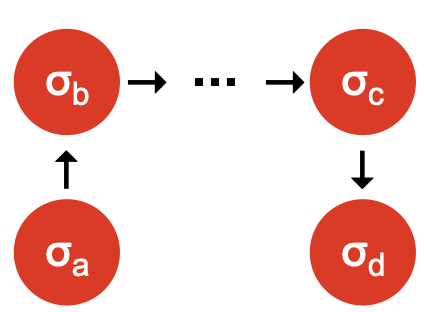
\includegraphics[width=\linewidth]{diagrams/compare.png}
} 
\end{minipage}
\end{tabular}
\end{flushleft}


{\emph{History  invariants}} \cite{liskov94behavioral,usinghistory,Cohen10}, instead, consider \sdred{all  future states including any method returns}, and therefore {would  require that   $\sigma_d \models A$. Thus, they are,}  for our purposes,  both
 \emph{unenforceable} and overly \emph{restrictive}.\ \  \emph{Unenforceable}: \ Take $A \txteq \inside{\prg{acc.key}}$,  assume  in $\sigma_a$ a path to an external object which has access to $\prg{acc.key}$, assume that path is unknown in $\sigma_b$: then, the transition from $\sigma_b$ to $\sigma_c$ cannot eliminate that path—hence, $\sigma_d \not\models \inside{\prg{acc.key}}$.\ \  \emph{Restrictive}:\ Take $A \txteq \inside{\prg{acc.key}}\wedge a.\prg{blnce}\geq b$; then,  requiring  $A$   to hold in all states from $\sigma_a$ until termination would prevent all future withdrawals from $a$, rendering the account useless.

{\emph{Object}} invariants  \cite{Meyer92,MeyerDBC92,BarDelFahLeiSch04,objInvars,MuellerPoetzsch-HeffterLeavens06}, on the other hand, expect %require -- too many require in the para
invariants to hold in all (visible) states,
here would require,  \eg that $\sigma_a \models A$. Thus, they  are %equally 
\emph{inapplicable} for us: They would require, \eg, that for all % objects 
 $\prg{acc}$, in all (visible) states, $\inside{\prg{acc.key}}$, and thus prevent \emph{any} withdrawals from \emph{any} account in \emph{any} state.
 


 

\paragraph{Discussion: The Difference between Postconditions and Invariants}
% The interested reader might have noticed that 
In all our method specification examples so far, the post-condition and the invariant part were identical.
However, this need not be so. 
Assume a method \prg{tempLeak} defined in \prg{Account}, with an external argument \prg{extArg}, and a method body:
\\
$\strut \hspace{1cm} \prg{extArg.m(this.key); this.key:=new Key}$
\\
Then, the assertion   $ \inside{\prg{this.key}}$  is  broken by the external call \prg{extArg.m(this.key)}, but is  established by \prg{his.key:=new Key}.
Therefore, $ \inside{\prg{this.key}}$  is not an invariant.
The specification of \prg{tempLeak} could be\\
$
{\sprepost
		{\strut \ \ \ \ \ \ \ \ \ S_{\prg{tempLeak}}} 
		{  \ \prg{true}\  }
		{\prg{public Account}} {\prg{tempLeak}} {\prg{extArg}:\prg{external}}
		{  \  \inside{\prg{this.key} }\  }
		{  \  \prg{true}\  }
}
$

 
 
\footnoteSD{First bullet: This means that we require all objects to satisfy even if not locally relevant. Second Bullet: notice that we are asking for globally relevant objects}  
\footnoteSD{{TODO: Make an example that demonstrates the difference if in the second bullet we had asked for locally relevant objects ${\overline o}$.}}
\footnoteSD{{TODO Notice that we assume that $\overline x$ are not free in $A$ -- cf Barendregt convention.}}
\footnoteSD{TODO: explain why we did not require the stronger $\leadstoFin{M_{ext}\!\circ \!M}{\sigma}{\sigma'}$ rather than $\leadstoBoundedStar {M_{ext}\!\circ \!M}{\sigma}  {\sigma'}$.}

\newcommand{\paragraphSDD}[1]{\vspace{.02cm}{\textit{#1}}}
 
\subsection{Expressiveness} 

We argue the expresseness of our approach  through a sequence of capability patterns studied in related approaches from the literature  
 \cite{OOPSLA22,dd,VerX,irisWasm23} written in our specification language.
These approaches %in  \cite{OOPSLA22,dd,VerX,irisWasm23}  
 are based on temporal logics \cite{VerX,OOPSLA22}, or on extensions of Coq/Iris \cite{dd,irisWasm23}, and
none offer a Hoare logic    for external calls.
%Other approaches in the literature are either unable to handle external method calls \cite{OOPSLA22}, or use  bespoke proofs \cite{dd,irisWasm23}, or model checking \cite{VerX}.
%Their specification languages are based on temporal logics \cite{VerX,OOPSLA22}, or on extensions of Coq and Iris \cite{dd,IrisWasm23}.
More in  \S \ref{app:expressivity}. 
% we argue our approach is able to prove comparable specifications to those proposed in  \cite{OOPSLA22,dd,VerX,irisWasm23}, in the presence of external method calls, using a Hoare logic.=≠≠≠q±±≠≠≠qq≠q≠≠www≠≠
We   summarize here.

 %% We continue the comparison of expresiveness between \emph{Chainmail} and \Nec, by 
 %% considering the examples studied in \cite{FASE}.
 
%\begin{example}[ERC20]

\paragraphSDD{DOM} % is the motivating example  in \cite{dd}:
Access to any DOM node
gives read/write  permissions to  all its \prg{parent} and \prg{children} nodes. 
These permissions are attenuated   through a \prg{Proxy} class, %which has a field \prg{node} pointing to a \prg{Node}, and a field \prg{height}, 
 which restricts the range of \prg{Node}s which may be modified through the use of the particular \prg{Proxy}. 
We  express such  attenuation   through two scoped invariants.
% The corresponding specification in \ref{OOPSLA22} is comparable, but not able to prove external calls. % not specific as to the frame from which any modification originated.

\paragraphSDD{DAO} %Decentralized Autonomous Organization\
 ~\cite{Dao}  is a well-known Ethereum contract   which was exploited with a re-entrancy bug in 2016, 
and lost \$50M. 
Our two state invariants  would have secured %the DAO 
 against that bug. % such a  bug. 
But note  that  they are about precluded effects, and 
%. They are, essentially, simple object invariants and 
thus expressible % could have been expressed 
 with techniques proposed in the 90's \cite{MeyerDBC92}.
% \cite{OOPSLA22}  gives one  further specification, which says  that any reduction of funds can only be caused through a call to a specific method -- such specifications are beoind our scope.
 
 \paragraphSDD{ERC20} is a widely used % token 
 standard describing  basic functionality of Ethereum-based token 
contracts. 
The Solidity security model is not based on access to  capabilities but on who the caller  is. 
We  adapted our approach correspondingly, and 
express 1) that  the owner of an account is always authorized on that account,  2) any execution which does not contain calls from a participant  authorized on some account will not affect the balance nor  who is authorized on  that account. 
% The specifications from \cite{OOPSLA22} are more API-specific, in that they pinpoint which method calls caused an effect, and less specific in that they do not pinpoint the frame from which the effect occurred. 

\paragraphSDD{Stack} is a Wasm module exporting separate functions to read or modify its contents \cite{irisWasm23}. We specify that in the absence of external access to the latter capability, the contents will not change.  


% already in the approach section  \begin{figure}[htb]
%\begin{tabular}{|c|}
%\hline  % \\
%\resizebox{7.3cm}{!}{
%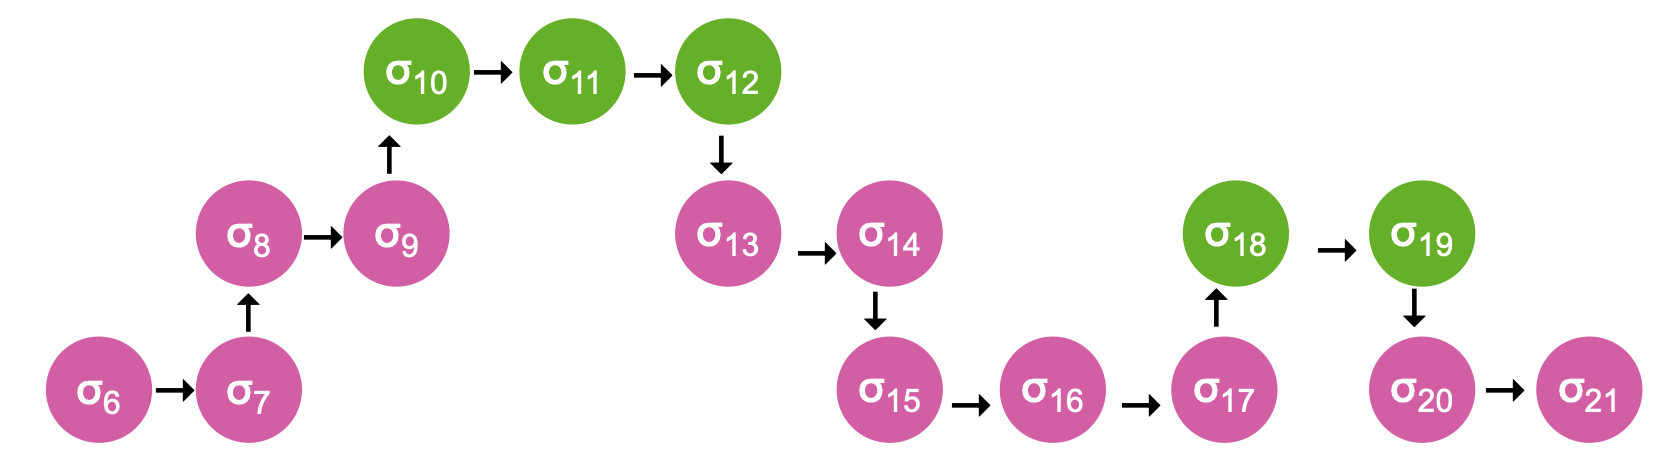
\includegraphics[width=\linewidth]{diagrams/preserves2.png}, 
%}
%\\
%\hline
%% \\
%\begin{tabular}{lcl}
%% not that interesting, chopped
%% $\leadstoBoundedStar {...} {\sigma_6}   {\sigma_9} $ & &  $A_0$ guaranteed to be preserved from $\sigma_6$ to $\sigma_9$.\\
%$\leadstoBoundedStar {...} {\sigma_6}   {\sigma_{13}} $ & &   $A_0$ guaranteed to be preserved from $\sigma_6$ to $\sigma_{13}$.\\
%$\leadstoBoundedStar {...} {\sigma_6}   {\sigma_{19}} $, \ \   $..,\sigma_{19}\not \models {\extThis} $ & &   $A_0$ \emph{not} guaranteed to be preserved from $\sigma_6$ to $\sigma_{19}$.\\
%$\leadstoBoundedStar {...} {\sigma_6}  {\sigma_{20}} $  \ \   & &  $A_0$  guaranteed to be preserved from $\sigma_6$ to $\sigma_{20}$.\\
%$\notLeadstoBoundedStar {...} {\sigma_8}  {\sigma_{20}} $  \ \   & &  $A_0$  \emph{not} guaranteed to be preserved from $\sigma_8$ to $\sigma_{20}$. \\
%\hline
%\end{tabular}
%\end{tabular}
%   \caption{Illustrating  the meaning on ${\TwoStatesN {\overline {x:C}} {A_0}}$  -- refining Fig. \ref{fig:UpSemantics}. }
%      \label{fig:illusrPreserve} 
% \end{figure}

%\move{
 %\begin{example}
 %\label{example:twostatesarisfy}
 %{We   revisit the specifications given in Sect. \ref{s:bankSpecEx}, and the one from Example \ref{example:twostate}, and  the three  modules from Sect. \ref{s:bank}:}
%
%
%\begin{tabular}{lllllllll}
%$\ModA  \models S_1$  &   $\ModA  \models S_2$ &  $\ModA \models S_3$ &   $\ModA \models S_4$    & $\ModA \models S_5$\\
% $\ModB \models S_1$  &   $\ModB \not\models S_2$   &  $\ModB  \models S_3$   &  $\ModB  \not\models S_4$   & $\ModB \not\models S_5$ \\
% $\ModC  \models S_1$    & $\ModC \models S_2$ &   $\ModC \models S_3$    &$\ModC \not\models S_4$   & $\ModC \not\models S_5$ 
%\end{tabular}
%\end{example}
 

 
 %\begin{example}
 %\label{example:mprepostlsatissy}
 %For  %method
 %Example \ref{example:mprepostl}, we have
 % $\ModA \models S_6$ and $\ModB \models S_6$ and  $\ModC \models S_6$.
%Also,  $\ModA \models S_7$ and $\ModB \models S_7$ and  $\ModC \models S_7$.
%However,   $\ModA  \models S_8$, while $\ModB  \not\models S_8$.
%\end{example}
%
 %\begin{example}
%\label{example:mprepostlsatissy}
 %For  %method
%any   specification  $S \triangleq {\mprepost{A}{p\ C}{m}{x}{C}{A'} }$ and any module  $M$ which does not have a class $C$  with a method $m$ with formal parameter  types ${\overline C}$, we have that $M \models S$.
%Namely, if a method were to be called with that signature on a $C$  from $M$, then execution would be stuck, and the requirements from Def. \ref{def:necessity-semantics}(3) would be trivially satisfied.
%Thus,   $\ModC \models S_8$. %, even though $\ModC$ does not have a method \prg{set} with the signature given in $S_6$;
%\end{example}
%}
 

%% KEEP ALL BELOW, but currently not needed 
%\subsection{\SpecLang Entailments}
%
%{We define entailment of specifications wrt a module in the expected way.} %The usual definition of entailment applies to our specifications as well}
%
%\begin{definition}[Satisfaction of Assertions by a module] 
%\label{def:assertion-inference-semantics}
%We define satisfaction of an assertion $A$ by a  module $M$ as:
%\begin{itemize}
%\item
%{
%$M \models A$   \ \ \ iff \ \ \  $\forall \overline{M}. \forall \sigma
%[\ \    \arising{\sigma}{M\madd\overline{M}}\   \  \wedge\ \  \satisfiesA {M}   {\sigma} {\external{\prg{this}}} 
%\   \ \Longrightarrow \ \ \satisfiesA{M}{\sigma}{A}\ \ ]$
%}\footnote{Not sure about the need for external and arising.}
%\end{itemize}
%\end{definition}
%
%%TODO: Here we will say that assertions are classical, as proven in FASE
%
%\begin{definition}[Stronger Specifications] 
%\label{def:specification-implication-semantics}
%Specification $S$ is stronger than another specification $S'$  in the context of a  module: 
% \begin{itemize}[itemsep=5pt]
%\item 
%$\stronger M  S  {S'}$   \ \ \ iff \ \ \  $M\models S$ implies $M \models S'$
%\item
%$\strongerEq M  S  {S'}$   \ \ \ iff \ \ \ $\stronger M  S  {S'}$  \ and \  $\stronger M   {S'} S$    
%\end{itemize}
%\end{definition}
%
%\noindent
%{Interestingly, entailment can deduce some method specifications out of two-state invariants.}
%
%{
% \begin{example}
% \label{example:entail}
% Any module $M$ whose code does not call  method \prg{buy} gives   $\stronger M {S_2 \wedge S_S4} {S_9}$
%\end{example}
%
%
%% Remember $S_1$, ... $S_4$ as defined in Sect. \ref{s:bankSpecEx}, and consider the specifications $S_6$ and $S_7$ from Example \ref{example:mprepostl}.
%% Then, for any module $M$ %which has a public method \prg{set}, 
%% we have that
%\begin{example}
% \label{example:entail}
%For any module $M$,  we have  $\strongerEq M {S_2 \wedge S_4} {S_2 \wedge S_{4a}}$, where $S_{4a}$ defined as 
%\\
%\begin{tabular}{lcll}
%  $S_{4a}$   & $\triangleq$   &  
% $ \TwoStatesQ{\prg{a}:\prg{Account},\prg{b}:\prg{int}}  {\inside{\prg{a.\password}} \wedge \prg{a.\balance}\geq\prg{b}} 
% {\inside{\prg{a.password}} \wedge \prg{a.\balance}\geq\prg{b}} $
% \end{tabular}
%\ \end{example}
%}
% 
%%Some properties of $M \models \_  \subseteq \_ $ are given below:
%%
%%\begin{lemma}
%%For assertions $A$, $A'$, variables $\overline y$, and $\overline x$, specifications $S$, $S'$, $S''$, and module $M$:
%%\begin{itemize} [topsep=6pt,itemsep=5pt,parsep=0pt,partopsep=0pt]
%%%\item
%%% $\stronger M {\OneStateQ {\overline {x:C}}  {A}}  {\TwoStatesQ {\overline {x:C}} {A}{A}} $ 
%%%    \item
%%%  $\strongerEq  M  {\OneStateQ    {y:\prg{Object}}   {\forall \overline {x:C}[ A ] } } 
%%%    {\OneStateQ {\overline {x:C}}  {A}} $.
%%\item
%%$\strongerEq M    {\TwoStatesQ {\overline {x:C}} {A}{A'}}    {\TwoStatesQ {\overline {y:C}} {A[y/x]}{A'[y/x]}}$
%%\item
%%$  M  \models    \overline {x:C} \wedge A_1'  \rightarrow A_1$ \ \ \  and \ \ \
%%$  M  \models  \overline {x:C} \wedge A_2'  \rightarrow A_2$  \ \ \ \ 
%%implies\\
%% $\strut \hspace{5cm} \stronger M  {\TwoStatesQ {\overline {x:C}} {A_1}{A_2}}     {\TwoStatesQ {\overline {x:C}} {A_1'}{A_2'}}$
%%
%%\item
%%$\stronger M  S {S''}$ and $\stronger M {S''} {S'}$\ \  \ implies\  \ \ $\stronger M S  {S'}$.
%%
%%\end{itemize}
%%
%%\end{lemma}


%%%%%%%%%%%%%%%%%%%%%%%%%%%%%%%%%%%%%%%%%%%%%%%%%%%%%%%%%%%%%%%%%%%%%%




% a state $\sigma$ is 
%{ an \emph{arising} state, formally \ \ \  $\arising{\sigma}{\Mtwo}$,\ \ \ if  there exists some $\sigma_0$ such that $\initial{\sigma_0}$ and
%$\Mtwo, {\sigma_0} \leadstoN^* {\sigma}$.}
%%\item
%%{A a state $\sigma$ is 
%%called an \emph{arising} state, formally\ \ \ \  $\extArising{\sigma}{M_{ext}}{M}$,\ \ \ \
%%if and only if $\arising{\sigma}{M_{ext}*M}$ and $M, \sigma \models \external{\prg{this}}$.}
%\end{itemize}
%\end{definition}
  
We now move to the semantics of specifications:   $M \models S$ expresses that  module  $M$   satisfies a specification  $S$.  
\sdN{For this, we fist define what it means for a state $\sigma$ to satisfy a triple of assertions:}

\sdN{
\begin{definition}
For modules $\Mtwo$, $M$, state $\sigma$, and assertions $A$, $A'$ and  $A''$, we define:
\begin{itemize}
\item
$ {\satAssertQuadruple  \Mtwo  M     {A} \sigma {A'} {A''} } \ \ \triangleq \ \ \forall \overline{\alpha}, \overline{z}, \sigma',\sigma''.[
$  \\
$\strut \hspace{.2cm} M,  \sigma \models  {A[\overline{\alpha/z}]}  % \, \wedge\,    {\GRelevant {\overline \alpha}  \sigma} 
  \  \ \Longrightarrow$\\
 $\strut   \ \ \ \  \  \ \ \ \   [ \ \ \  {\leadstoBoundedStarFin { \Mtwo\madd M}{\sigma}  {\sigma'} }\ \ \Longrightarrow\ \   M,  \sigma' \models  {A'[\overline{\alpha/z}]}  \ \ \ \  ] \ \ \ \wedge$\\
 $\strut   \ \ \ \  \  \ \ \ \   [ \ \  \ {\leadstoBoundedStar  {\Mtwo\madd M}{\sigma}  {\sigma''} }\ \  \ \Longrightarrow\   \   M,  \sigma'' \models  {(\extThis \rightarrow A''[\overline{\alpha/z}])} \ \ \  ] $\\
 $\strut \hspace{.2cm}$ where  ${\red{\overline z= \fv(A)\!\setminus\! \vs(\sigma.\prg{cont})}}  \ \ \ ]$ %\ \ \ \  \ \ \ \  \ \  \ \ \ \  \ \ \ \ ]$
\end{itemize}
\end{definition}
}


\begin{definition}  [Semantics of  Specifications]
We define $\satisfies{M}{{S}}$ by cases over the three possible syntactic forms.

\label{def:necessity-semantics}

\begin{enumerate}
 \item
 $\satisfies{M}{\TwoStatesN {\overline {x:C}} {A}} \ \  \ \triangleq   \ \ \ \sdN{\forall   \Mtwo,  \sigma.[\ {\satAssertQuadruple  \Mtwo  M    {\extThis \wedge \overline {x:C} \wedge A} \sigma {A} {A} }\ ].}$
  \item
 $\satisfies{M} { \mprepostN {A_1}{p\ D}{m}{y}{D}{A_2} {A_3} }\  \ \ \   \triangleq    \ \ \ \forall   \Mtwo,  \sigma.[\ $    \\
$\strut  \ \ \   \ \ \ \ \ \ \ \ \   \   \sdN{ \forall   y_0,\overline y, \sigma[ \ \ \ \sigma\txteq {u:=y_0.m(y_1,..y_n)} \ \ \Longrightarrow \ \ 
\satisfies  {M} {\quadruple  {A_1'} }   {\sigma}   {A_2' } {A_3' }  \  \ \  ]} $  \\
$\strut  \ \ \   \ \ \ \ \ \ \ \ \   \  \mbox{where}$\\
$\strut  \ \ \   \ \ \ \ \ \ \ \ \   \   A_1' \triangleq   y_0:D,{\overline {y:D}}   \wedge   A[y_0/\prg{this}],\  \  A_2' \triangleq A_2[u/res,y_0/\prg{this}],\ \ A_3' \triangleq A_3[y_0/\prg{this}]   \  ]$  
 \item
 $\satisfies{M}{S\, \wedge\, S'}$\ \ \  \ \ \  $\triangleq$  \  \ \  \   $\satisfies{M}{S}\ \wedge \ \satisfies{M}{S'}$
\end{enumerate}
\end{definition}


\footnoteSD{First bullet: This means that we require all objects to satisfy even if not locally relevant. Second Bullet: notice that we are asking for globally relevant objects}  
\footnoteSD{{TODO: Make an example that demonstrates the difference if in the second bullet we had asked for locally relevant objects ${\overline o}$.}}
\footnoteSD{{TODO Notice that we assume that $\overline x$ are not free in $A$ -- cf Barendregt convention.}}
\footnoteSD{TODO: explain why we did not require the stronger $\leadstoFin{M_{ext}\!\circ \!M}{\sigma}{\sigma'}$ rather than $\leadstoBoundedStar {M_{ext}\!\circ \!M}{\sigma}  {\sigma'}$.}
% Note that the requirements that $\extArising{\sigma}{M_{ext}}{M}$ and $\leadstoFin{M_{ext}\circ M}{\sigma}{\sigma'} $ imply that
% $M, \sigma' \models {\external{\prg{this}}}$



We demonstrate the meaning of ${\TwoStatesN {\overline {x:C}} {A}}$ in Fig. \ref{fig:illusrPreserve} where we refine the execution shown in Fig. \ref{fig:UpSemantics}, and take it that the pink states, \ie   ${\sigma_6}$-${\sigma_9}$ and $\sigma_{13}$-$\sigma_{17}$, and  $\sigma_{20}$, $\sigma_{21}$ are external, and the green states, \ie   ${\sigma_{10}}$,  ${\sigma_{11}}$,   ${\sigma_{12}}$,  ${\sigma_{18}}$, and  ${\sigma_{19}}$, are internal. 
 
 \begin{figure}[htb]
\begin{tabular}{|c|}
\hline  % \\
\resizebox{8cm}{!}{
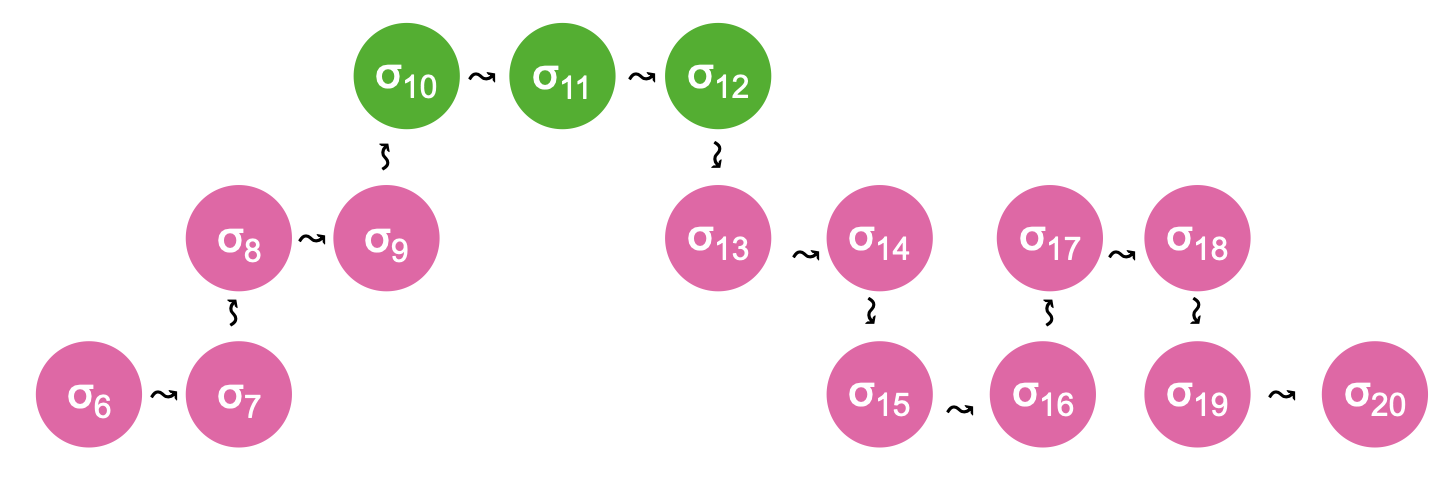
\includegraphics[width=\linewidth]{diagrams/preserves.png}, 
} 
\\
\hline
% \\
\begin{tabular}{lcl}
$\leadstoBoundedStar {...} {\sigma_6}   {\sigma_9} $ & & thus, $A_0$ guaranteed to be preserved from $\sigma_6$ to $\sigma_9$.\\
$\leadstoBoundedStar {...} {\sigma_6}   {\sigma_{13}} $ & & thus, $A_0$ guaranteed to be preserved from $\sigma_6$ to $\sigma_{13}$.\\
$\leadstoBoundedStar {...} {\sigma_6}   {\sigma_{19}} $, \ \  but $..,\sigma_{19}\not \models {\external{\prg{this}}}$ & & thus, $A_0$ not guaranteed to be preserved from $\sigma_6$ to $\sigma_{19}$.\\
$\leadstoBoundedStar {...} {\sigma_6}  {\sigma_{20}} $  \ \   & & thus, $A_0$  guaranteed to be preserved from $\sigma_6$ to $\sigma_{20}$.\\
$\notLeadstoBoundedStar {...} {\sigma_8}  {\sigma_{20}} $  \ \   & & thus, $A_0$  not guaranteed to be preserved from $\sigma_8$ to $\sigma_{20}$.\\
\hline
\end{tabular}
\end{tabular}
   \caption{Illustrating  the meaning on ${\TwoStatesN {\overline {x:C}} {A_0}}$  -- refining Fig. \ref{fig:UpSemantics}. }
      \label{fig:illusrPreserve} 
 \end{figure}
 
 \begin{example}
 \label{example:twostatesarisfy}
 {We   revisit the specifications given in Sect. \ref{s:bankSpecEx}, and the one from Example \ref{example:twostate}, and  the three  modules from Sect. \ref{s:bank}:}


\begin{tabular}{lllllllll}
$\ModA  \models S_1$  &   $\ModA  \models S_2$ &  $\ModA \models S_3$ &   $\ModA \models S_4$    & $\ModA \models S_5$\\
 $\ModB \models S_1$  &   $\ModB \not\models S_2$   &  $\ModB  \models S_3$   &  $\ModB  \not\models S_4$   & $\ModB \not\models S_5$ \\
 $\ModC  \models S_1$    & $\ModC \models S_2$ &   $\ModC \models S_3$    &$\ModC \not\models S_4$   & $\ModC \not\models S_5$ 
\end{tabular}
\end{example}
 

 
 \begin{example}
 \label{example:mprepostlsatissy}
 For  %method
 Example \ref{example:mprepostl}, we have
  $\ModA \models S_6$ and $\ModB \models S_6$ and  $\ModC \models S_6$.
Also,  $\ModA \models S_7$ and $\ModB \models S_7$ and  $\ModC \models S_7$.
However,   $\ModA  \models S_8$, while $\ModB  \not\models S_8$.
\end{example}

 \begin{example}
\label{example:mprepostlsatissy}
 For  %method
any   specification  $S \triangleq {\mprepost{A}{p\ C}{m}{x}{C}{A'} }$ and any module  $M$ which does not have a class $C$  with a method $m$ with formal parameter  types ${\overline C}$, we have that $M \models S$.
Namely, if a method were to be called with that signature on a $C$  from $M$, then execution would be stuck, and the requirements from Def. \ref{def:necessity-semantics}(3) would be trivially satisfied.
Thus,   $\ModC \models S_8$. %, even though $\ModC$ does not have a method \prg{set} with the signature given in $S_6$;
\end{example}

 

%% KEEP ALL BELOW, but currently not needed 
%\subsection{\SpecLang Entailments}
%
%{We define entailment of specifications wrt a module in the expected way.} %The usual definition of entailment applies to our specifications as well}
%
%\begin{definition}[Satisfaction of Assertions by a module] 
%\label{def:assertion-inference-semantics}
%We define satisfaction of an assertion $A$ by a  module $M$ as:
%\begin{itemize}
%\item
%{
%$M \models A$   \ \ \ iff \ \ \  $\forall \overline{M}. \forall \sigma
%[\ \    \arising{\sigma}{M\madd\overline{M}}\   \  \wedge\ \  \satisfiesA {M}   {\sigma} {\external{\prg{this}}} 
%\   \ \Longrightarrow \ \ \satisfiesA{M}{\sigma}{A}\ \ ]$
%}\footnote{Not sure about the need for external and arising.}
%\end{itemize}
%\end{definition}
%
%%TODO: Here we will say that assertions are classical, as proven in FASE
%
%\begin{definition}[Stronger Specifications] 
%\label{def:specification-implication-semantics}
%Specification $S$ is stronger than another specification $S'$  in the context of a  module: 
% \begin{itemize}[itemsep=5pt]
%\item 
%$\stronger M  S  {S'}$   \ \ \ iff \ \ \  $M\models S$ implies $M \models S'$
%\item
%$\strongerEq M  S  {S'}$   \ \ \ iff \ \ \ $\stronger M  S  {S'}$  \ and \  $\stronger M   {S'} S$    
%\end{itemize}
%\end{definition}
%
%\noindent
%{Interestingly, entailment can deduce some method specifications out of two-state invariants.}
%
%{
% \begin{example}
% \label{example:entail}
% Any module $M$ whose code does not call  method \prg{buy} gives   $\stronger M {S_2 \wedge S_S4} {S_9}$
%\end{example}
%
%
%% Remember $S_1$, ... $S_4$ as defined in Sect. \ref{s:bankSpecEx}, and consider the specifications $S_6$ and $S_7$ from Example \ref{example:mprepostl}.
%% Then, for any module $M$ %which has a public method \prg{set}, 
%% we have that
%\begin{example}
% \label{example:entail}
%For any module $M$,  we have  $\strongerEq M {S_2 \wedge S_4} {S_2 \wedge S_{4a}}$, where $S_{4a}$ defined as 
%\\
%\begin{tabular}{lcll}
%  $S_{4a}$   & $\triangleq$   &  
% $ \TwoStatesQ{\prg{a}:\prg{Account},\prg{b}:\prg{int}}  {\inside{\prg{a.\password}} \wedge \prg{a.\balance}\geq\prg{b}} 
% {\inside{\prg{a.password}} \wedge \prg{a.\balance}\geq\prg{b}} $
% \end{tabular}
%\ \end{example}
%}
% 
%%Some properties of $M \models \_  \subseteq \_ $ are given below:
%%
%%\begin{lemma}
%%For assertions $A$, $A'$, variables $\overline y$, and $\overline x$, specifications $S$, $S'$, $S''$, and module $M$:
%%\begin{itemize} [topsep=6pt,itemsep=5pt,parsep=0pt,partopsep=0pt]
%%%\item
%%% $\stronger M {\OneStateQ {\overline {x:C}}  {A}}  {\TwoStatesQ {\overline {x:C}} {A}{A}} $ 
%%%    \item
%%%  $\strongerEq  M  {\OneStateQ    {y:\prg{Object}}   {\forall \overline {x:C}[ A ] } } 
%%%    {\OneStateQ {\overline {x:C}}  {A}} $.
%%\item
%%$\strongerEq M    {\TwoStatesQ {\overline {x:C}} {A}{A'}}    {\TwoStatesQ {\overline {y:C}} {A[y/x]}{A'[y/x]}}$
%%\item
%%$  M  \models    \overline {x:C} \wedge A_1'  \rightarrow A_1$ \ \ \  and \ \ \
%%$  M  \models  \overline {x:C} \wedge A_2'  \rightarrow A_2$  \ \ \ \ 
%%implies\\
%% $\strut \hspace{5cm} \stronger M  {\TwoStatesQ {\overline {x:C}} {A_1}{A_2}}     {\TwoStatesQ {\overline {x:C}} {A_1'}{A_2'}}$
%%
%%\item
%%$\stronger M  S {S''}$ and $\stronger M {S''} {S'}$\ \  \ implies\  \ \ $\stronger M S  {S'}$.
%%
%%\end{itemize}
%%
%%\end{lemma}


%%%%%%%%%%%%%%%%%%%%%%%%%%%%%%%%%%%%%%%%%%%%%%%%%%%%%%%%%%%%%%%%%%%%%%


